Ce chapitre décrit les choix qui ont été faits pour implémenter l'algorithme développé dans le chapitre \ref{pro}. La section \ref{sec:lprog} présente les choix envisagés de langages de programmation et librairies avant de nommer le candidat retenu de façon argumentée.
Ensuite, la section \ref{sec:diffs} décrit les difficultés rencontrées ainsi que les solutions et compromis apportés à chacune d'elles. Trois d'entre elles étaient de l'ordre algorithmique. Les algorithmes proposés sont expliqués dans les sections \ref{sec:app}, \ref{sec:fl} et \ref{sec:fll}. Chacun est accompagné d'un exemple.
Finalement, quelques expérimentations sont citées et appréciées dans la section \ref{sec:exps}.

Un résumé des changements effectués dans les librairies utilisées est disponible dans l'annexe \ref{app:mods}.

\section{Langage de programmation et librairies}\label{sec:lprog}Implémenter ces différents types d'automates, les opérations associées, ainsi que les différents algorithmes demande une quantité considérable de travail.

Utiliser des librairies pré-existantes permet de réutiliser du code et de limiter le travail restant, plus spécifique à ce document.

Une librairie en python, \href{https://pypi.org/project/automata-lib/}{automata-lib} ainsi que les librairies java \href{https://learnlib.de/projects/automatalib/}{Automatalib} et \href{https://learnlib.de/}{Learnlib} ont été considérées.

automata-lib supporte tous les types d'automates necéssaires, avec des méthodes de bases telles que l'exécution pour un mot, la validité pour les automates sans files ainsi qu'une méthode de construction simple. Cependant, il manque beaucoup de fonctionnalités. Les opérations booléennes entre automates ne sont pas implémentées. La déterminisation d'un NFA ou l'algorithme d'Angluin ne sont pas proposés non plus.

Pour ces raisons, le couple Automatalib-Learnlib a été retenu. Ces librairies sont plus complexes et ne supportent pas les automates à files. Cependant, toutes les autres opérations citées précédemment sont présentes. Cela permet de limiter le travail à l'implémentation des automates à files et des méthodes et algorithmes couverts dans les chapitres \ref{pro} et \ref{impl}.

\section{Difficultés}\label{sec:diffs}Ce travail a rencontré plusieurs difficultés. En voici la liste avec les contre-mesures proposées si c'est pertinent.

\begin{itemize}
  \item Les librairies utilisées sont complexes. Automatalib et Learnlib sont conçues de façon très générique. Cependant, ajouter le concept de file aux automates n'était pas prévu. La solution apportée est de développer un pan dans chaque librairie dédié plus spécifiquement aux automates à files. Éventuellement, des méthodes ont été dupliquées dans ce contexte.
  \item La documentation était insuffisante ou introuvable. La documentation des librairies sur leur site respectif est succinte et sommaire. En général, le code n'est commenté que pour les classes n'ayant pas elles-même de super-classe. De plus, il manque des explications sur les relations entre les classes. Pour travailler dans ces conditions, il a fallu explorer une grande partie du projet, tester certaines fonctionnalités. Pour simplifier la lecture du code ajouté, des commentaires plus fréquents y ont été ajoutés. L'annexe \ref{app:mods} sert aussi de référence aux relations entre classes.
  \item Certaines opérations ne sont proposées que pour les ANF alors que l'algorithme d'Angluin est défini ici pour les ADF. Une fonctionnalité a été ajoutée pour la traduction triviale d'un ANF à un ADF équivalent.
  \item Les librairies utilisent des dépendances complexes. Chaque librairie est découpée en de nombreux sous-modules interconnectés. Les cycles de dépendances sont interdits entre autres pour l'interprétation des annotations et la génération de code. La structure en sous-modules n'a pas été modifiée mais une attention particulière a été apportée aux dépendances et aux fichiers de configuration. Cette complexité se traduit aussi par un processus de compilation complexe.
  \item L'article de Vardhan et al.\cite{Vardhan04} manque de précision sur l'implémentation de la méthode \emph{LeVer}. La comparaison d'ensembles potentiellement infinis (les langages) manque d'explications sur la mise en pratique avec les automates. Des algorithmes ont dû être reconstruits pour permettre l'implémentation de ces opérations sur des ordinateurs. Parmis ceux-ci :
  \begin{itemize}
    \item L'algorithme d'appartenance de la section \ref{sec:app}.
    \item L'algorithme permettant de calcul de $\mathcal{F}(L)$ pour un langage de traces annotées $L$ donné, à la section \ref{sec:fl}
    \item L'algorithme permettant de comparer \fl et $L$ pour trouver un contre-exemple prouvant que $L$ n'est pas un point-fixe de $\mathcal{F}$, à la section \ref{sec:fll}.
  \end{itemize}
  L'article ne détaille pas non plus d'algorithme permettant de calculer l'ensemble des configurations à risque $\mathcal{W}(L)$. Cet ensemble est plus facile à calculer si les langages réguliers décrivant les configurations à risques ne s'intéressent pas au contenu des canaux mais uniquement aux états traversés dans l'automate à files. C'est cette approche qui est utilisée dans ce travail.
\end{itemize}

Une solution idéale à toutes ces difficultés demanderait une réécriture profonde des librairies ainsi qu'un grand travail de documentation. Cela améliorait grandement la qualité du code mais est au-delà des limites de ce travail.

\section{Algorithme d'appartenance}\label{sec:app}Les automates à files définis à la section \ref{fifo} sont plus puissants que les ADF définis dans la section \ref{adf}. En effet, les systèmes de transitions associés ont potentiellement une infinité de configurations. Dans ces conditions, il n'est pas possible de faire une exploration exhaustive des états pour trouver lesquels sont acceptants.

À la place, une propriété dite de sécurité est définie. Si un état respecte cette propriété, il est \emph{sûr}. Si il y a moyen de prouver que la totalité des états de l'automate respectent cette propriété, l'automate est considéré comme sûr. Si au contraire, un exemple de violation de la propriété est trouvé, l'automate peut être déclaré comme à risque.

L'idée dès lors est de travailler non pas avec un système de transitions infini mais avec une représentation construite pour être finie dans un vaste ensemble de problèmes. Cette représentation est le langage de trace défini dans la section \ref{trace}.

En supposant que celui-ci est régulier, il est possible d'utiliser l'algorithme d'Angluin de la section \ref{angluin} pour l'apprendre. Cependant, ce langage n'est qu'un concept et le professeur n'a accès qu'à un automate à files $F$. Pour cette raison, les oracles d'appartenance et d'équivalence sont adaptés pour répondre à une requête entre un langage fourni par l'élève et $F$.

La figure \ref{fig:lever} donne une vue schématique de ce nouvel algorithme d'Angluin modifié.


\begin{figure}[H]
	\centering

	\resizebox{\textwidth}{!}{
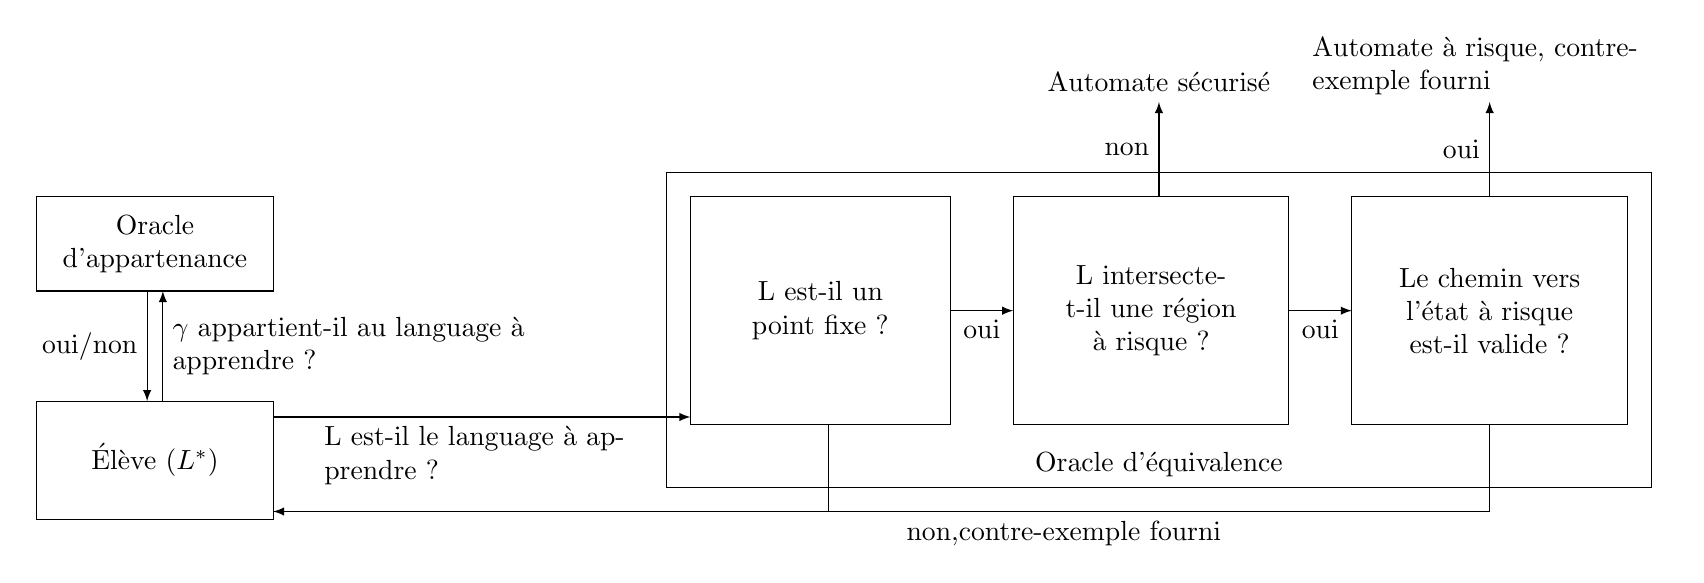
\begin{tikzpicture}
	\tikzset{>=latex}

  \draw (-3,-2.9) rectangle (0,-4.4) node[pos=.5] {Élève ($L^*$)};
  \draw (5,0) rectangle (17.5,-4);
	\draw[->] (0,-3.1) -- (5.3,-3.1) node[pos=0.5,below,text width=4cm] {L est-il le language à apprendre ?};

  \draw (-3,-0.3) rectangle (0,-1.5) node[pos=.5,text width=3cm,align=center] {Oracle\\ d'appartenance};
  \draw[->] (-1.4,-2.9) -- (-1.4,-1.5) node[pos=0.5,right,text width=5cm] {$\gamma$ appartient-il au language à apprendre ?};
  \draw[<-] (-1.6,-2.9) -- (-1.6,-1.5) node[pos=0.5,left] {oui/non};

  \node[draw=none] at (11.25, -3.7) {Oracle d'équivalence};

  \draw (5.3, -0.3) rectangle (8.6, -3.2) node[pos=0.5,text width=3cm,align=center] {L est-il un point fixe ?};
  \draw (9.4, -0.3) rectangle (12.9, -3.2) node[pos=0.5,text width=3cm,align=center] {L intersecte-t-il une région à risque ?};
  \draw (13.7, -0.3) rectangle (17.2, -3.2) node[pos=0.5,text width=3cm,align=center] {Le chemin vers l'état à risque est-il valide ?};

  \draw[->] (8.6, -1.75) -- (9.4,-1.75) node[pos=0.5,below] {oui};
  \draw[->] (12.9, -1.75) -- (13.7,-1.75) node[pos=0.5,below] {oui};
  \draw[->] (15.45, -4.3) -- (0, -4.3) node[pos=0.35,below] {non,contre-exemple fourni};
  \draw[-] (7.05, -3.2) -- (7.05, -4.3);
  \draw[-] (15.45, -3.2) -- (15.45, -4.3);

	\draw[->] (11.25,-0.3) -- (11.25,0.9)node[pos=0.5,left] {non};
	\draw[->] (15.45,-0.3) -- (15.45,0.9)node[pos=0.5,left] {oui};

	\node[draw=none] at (11.25, 1.15) {Automate sécurisé};
	\node[draw=none,text width=4.5cm] at (15.45, 1.36) {Automate à risque, contre-exemple fourni};


\end{tikzpicture}
}
\caption{Vue schématique de l'algorithme d'Angluin pour LeVer\cite{Vardhan04}}\label{fig:lever}
\end{figure}


\emph{LeVer} est le nom de cette technique. En particulier, on peut noter sur ce schéma que l'oracle d'équivalence peut non seulement répondre oui ou non mais également interrompre l'apprentissage s'il est possible de se prononcer sur la sûreté d'un automate à files $F$. Pour rappel, $L(F)$ n'est pas régulier en général. Pouvoir se prononcer sur la sûreté de $F$ étant possible, il n'est ni utile ni forcémment possible de continuer à appliquer $L^*$ pour obtenir une meilleure approximation $L$ du langage de trace de $F$. 

\section{Algorithme de construction de $\mathcal{F}(L)$}\label{sec:fl}Soit un langage $L$ et un automate $A$ tel que $L=L(A)$. Calculer $\mathcal{F}(L)$ revient, par définition, à calculer $\bigcup_{\theta\in\Theta}Post(L,\theta)\bigcup \{t_{q_0}\}$.

Pour rappel, voici la définition de $Post(L, \theta)$ telle que donnée dans la section \ref{trace:extension} :

$Post(L,\theta)=\bigcup_{\gamma\in L} Post(\gamma,\theta)$ avec

$$
Post(\gamma,\theta) = \left\{ \begin{array}{ll}
    \emptyset & \text{si } \gamma \text{ n'est pas correctement formaté ou si } \mathcal{C}(\gamma)\neq source(\theta)\\
    \{\mathcal{T}(\gamma)t_{cible(\theta)}\} & \text{sinon si }\delta(\theta)=(p,\tau,q) \text{ ou } \delta(\theta)=(p,c_i!a_j,q) \text{ avec }p,q\in Q\\
    \{deriv(\mathcal{T}(\gamma),\theta)t_{cible(\theta)}\}& \text{sinon si } \delta(\theta)=(p,c_i?a_j,q) \text{ avec }p,q\in Q \\
    \end{array} \right.
$$

Des automates $A_\theta$ peuvent être construits pour $Post(L,\theta)$ pour chaque $\theta$ à partir de $A$. L'union de ces automates $A'=\bigcup_{\theta \in \Theta A_\theta}$ accepte $\bigcup_{\theta\in\Theta}Post(L,\theta)$. L'union de ce nouvel automate avec un automate pour le language $L=\{t_{q_0}\}$ accepte $\mathcal{F}(L)$.

La suite de cette section s'intéresse donc au calcul de $L'= Post(L,\theta)$ où $L$ est accepté par $A$ et $L'$ par un ADF $A'$ construit à partir de $A$.\\

L'automate $A'$ peut être non-déterministe. Ce n'est pas un problème car, comme l'explique la section \ref{adf:anfadf}, il existe un ADF équivalent. Dans le cadre de l'apprentissage avec Angluin, c'est cet ADF qui devient $A'$ et est utilisé pour les autres opérations.


Soit $\theta\in\Theta$ tel que $\delta(\theta)=(p,action,q)$. On explique ci-après les différents cas à traiter pour calculer $A_\theta$.

\subsection{Si $action$ est $\tau$ ou de la forme $c!a$}

Dans ce cas, construire un automate pour $L'=L\bigcap\Sigma^*t_p$ avec $t_p$ correspondant au $p$ de $\delta(\theta)$ et $\Sigma^*t_p$ étant représenté par l'ANF de la figure \ref{fig:sigmatq}.

\begin{figure}[H]
    \centering
    \begin{tikzpicture}[->,>=stealth',shorten >=1pt,auto,node distance=3cm, semithick, bend angle=10]
    \tikzstyle{every state}=[circle,scale=0.5]
    \node[state] (0) {};
    \node[state,accepting] (1)   [right of=0] {};

    \path
    (0) edge[loop above] node {$\Sigma$} (0)
    (0) edge node {$t_p$} (1)
    ;
    \end{tikzpicture}
    \caption{ANF pour $L=\Sigma^*t_p$}\label{fig:sigmatq}
\end{figure}


Dans cet automate $L'$, seuls les états et transitions menant à l'état final par $t_p$ sont considérés.

Construire un automate pour $L\bigcap\Sigma^*t_p=L'$. Si $L'$ est vide, c'est qu'il n'y a pas de mot finissant concerné par $\theta$ et donc que $Post(L,\theta)=\emptyset$.

Sinon, si $L'\neq\emptyset$, supposons d'abord que $action$ est de la forme $c!a$ ou $\tau$. Il faut alors appliquer une transformation à l'automate correspondant à $Post(L',\theta)$.
Si $action$ est de forme $c!a$, la transition sur $\theta$ peut être ajoutée avant les transitions sur $t_p$ et un nouveau $t_q$ signalant le changement d'état dans l'automate à files $F$.

\begin{figure}[H]
    \centering
    \begin{subfigure}{0.5\linewidth}
        \centering
        \begin{tikzpicture}[->,>=stealth',shorten >=1pt,auto,node distance=3cm, semithick, bend angle=10]
            \tikzstyle{every state}=[circle,scale=0.5]
            \node[state] (0) {};
            \node[state,accepting] (1)   [right of=0] {};
            \node[ellipse] [left of=0] {};
            \path
            (0) edge node {$t_p$} (1)
            ;
            \draw (-1,0) ellipse[x radius=1.5,y radius=1];
        \end{tikzpicture}
        \caption{Automate de $L'$}
    \end{subfigure}\hfill
    \begin{subfigure}{0.5\linewidth}
        \centering
        \begin{tikzpicture}[->,>=stealth',shorten >=1pt,auto,node distance=3cm, semithick, bend angle=10]
            \tikzstyle{every state}=[circle,scale=0.5]
            \node[state] (0) {};
            \node[state] (1) [right of=0] {};
            \node[state,accepting] (2)   [right of=1] {};

            \path
            (0) edge node {$\theta$} (1)
            (1) edge node {$t_q$} (2)
            ;
            \draw (-1,0) ellipse[x radius=1.5,y radius=1];
        \end{tikzpicture}
        \caption{Automate de $Post(L',\theta)$}
    \end{subfigure}
    \caption{Application de $Post(L',\theta)$ sur un automate si l'action est de forme $c!a$}
\end{figure}

À présent, supposons que l'action de $\theta$ est de forme $\tau$, $\theta\notin\Phi$. Alors, $t_p$ est remplacé par $t_q$. La transition est alors sous-entendue.

\begin{figure}[H]
    \centering
    \begin{subfigure}{0.5\linewidth}
        \centering
        \begin{tikzpicture}[->,>=stealth',shorten >=1pt,auto,node distance=3cm, semithick, bend angle=10]
            \tikzstyle{every state}=[circle,scale=0.5]
            \node[state] (0) {};
            \node[state,accepting] (1)   [right of=0] {};
            \node[ellipse] [left of=0] {};
            \path
            (0) edge node {$t_p$} (1)
            ;
            \draw (-1,0) ellipse[x radius=1.5,y radius=1];
        \end{tikzpicture}
        \caption{Automate de $L'$}
    \end{subfigure}\hfill
    \begin{subfigure}{0.5\linewidth}
        \centering
        \begin{tikzpicture}[->,>=stealth',shorten >=1pt,auto,node distance=3cm, semithick, bend angle=10]
            \tikzstyle{every state}=[circle,scale=0.5]
            \node[state] (0) {};
            \node[state,accepting] (1)   [right of=0] {};
            \node[ellipse] [left of=0] {};
            \path
            (0) edge node {$t_q$} (1)
            ;
            \draw (-1,0) ellipse[x radius=1.5,y radius=1];
        \end{tikzpicture}
        \caption{Automate de $Post(L',\theta)$}
    \end{subfigure}
    \caption{Application de $Post(L',\theta)$ sur un automate si l'action est $\tau$}
\end{figure}


\subsection{Si $action$ est de la forme $c?a$}

Pour qu'une réception $c?a$ d'un symbole soit possible, il faut qu'il existe un envoi qui lui soit associé. Cet envoi est noté $\theta_s$ tel que $\delta(\theta_s)=(r,c!a,s)$. De plus, il faut, comme dans la section précédente, tester si $Post(L,\theta)$ est vide ou non grâce au $t_p$ correspondant au $p$ de $\delta(\theta)$.

En utilisant $\theta_s$, on construit $L'=L\bigcap\Sigma^*\Theta_s\Sigma^*t_p$ où $\Theta_s$ est l'ensemble des $\theta_s$ associés à $c?a$. Un automate acceptant ce langage est donné à la figure \ref{fig:lseconde}.

\begin{figure}[H]
    \centering
    \begin{tikzpicture}[->,>=stealth',shorten >=1pt,auto,node distance=3cm, semithick, bend angle=10]
        \tikzstyle{every state}=[circle,scale=0.5]
        \node[state] (0) {};
        \node[state] (1) [right of=0] {};
        \node[state,accepting] (2)   [right of=1] {};

        \path
        (0) edge[loop above] node {$\Sigma$} (0)
        (0) edge node {$\Theta_s$} (1)
        (1) edge[loop above] node{$\Sigma$} (1)
        (1) edge node {$t_p$} (2)
        ;
    \end{tikzpicture}
    \caption{ANF pour $L=\Sigma^*\Theta_s\Sigma^*t_p$}\label{fig:lseconde}
\end{figure}

Si $L'=\emptyset$, il n'existe pas de $\theta_s$ dans les chemins qui nous concernent. Il n'y aura donc pas de possibilité de consommer un symbole : $Post(L,\theta)=\emptyset$.

Sinon si $L'$ est non vide, il faut alors, à partir de l'automate $A'$ acceptant $L'$, construire un automate $A_\theta$ acceptant le langage $Post(L',\theta)$.

\begin{figure}[H]
    \centering
    \begin{tikzpicture}[->,>=stealth',shorten >=1pt,auto,node distance=3cm, semithick, bend angle=10]
        \tikzstyle{every state}=[circle,scale=0.5]
        \node[state] (0) {$r$};
        \node[state] (1) [right of=0] {$s$};

        \node[state] (2) [right=4.5cm of 0] {$r'$};
        \node[state] (3) [right of=2] {$s'$};

        \path
        (0) edge[bend right=30] node {$\bt_s$} (3)
        (2) edge node {$\theta_s$} (3)
        ;
        \path [dashed]
        (0) edge node {$\theta_s$} (1)
        ;
        \draw (-1,-1.5) rectangle ++(3,3);
        \draw (4,-1.5) rectangle ++(3,3);

        \node at(0.5,-2) {$A'$};
        \node at(5.5,-2) {$A'_{copie}$};

    \end{tikzpicture}
    \caption{Première étape de construction de l'automate $P_A$ pour $Post(L'',\theta)$}\label{fig:aaprime}
\end{figure}

La figure \ref{fig:aaprime} décrit comment l'automate $A_\theta$ est construit à partir de $A'$. Premièrement, une copie de $A'$ est construite : $A'_{copie}$.
Dans $A'$, les états finaux sont considérés comme des états non finaux. Dans $A'_{copie}$, l'état initial est considéré comme un état non initial. Finalement, dans $A'$, toute transition $\theta_s$ allant de $r$ à $s$ est remplacée par une transition sur $\bt_s$ allant de $r$ à $s'$.

De cette façon, pour qu'un mot soit valide, il faut qu'il commence dans $A'$. La première occurence de $\theta_s$ a été systématiquement remplacée pour $\bt_s$ menant à $A'_{copie}$. Dans $A'_{copie}$, les autres transitions ne sont pas modifiées, laissant intact le reste du chemin. Cependant, la figure \ref{fig:aaprime} à elle seule ne suffit pas à construire $A_\theta$. Pour rester en accord avec la définition de $Post(L,\theta)$, il faut adapter le dernier symbole, ici $t_p$ en $t_q$ (figure \ref{fig:pq}).


\begin{figure}[H]
    \centering
    \begin{subfigure}{0.5\linewidth}
        \centering
        \begin{tikzpicture}[->,>=stealth',shorten >=1pt,auto,node distance=3cm, semithick, bend angle=10]
            \tikzstyle{every state}=[circle,scale=0.5]
            \node[state] (0) {};
            \node[state,accepting] (1)   [right of=0] {};
            \path
            (0) edge node {$t_p$} (1)
            ;
            \draw (-2,-1) rectangle ++(4,2);
        \end{tikzpicture}
        \caption{Automate de la figure \ref{fig:aaprime}}
    \end{subfigure}\hfill
    \begin{subfigure}{0.5\linewidth}
        \centering
        \begin{tikzpicture}[->,>=stealth',shorten >=1pt,auto,node distance=3cm, semithick, bend angle=10]
            \tikzstyle{every state}=[circle,scale=0.5]
            \node[state] (0) {};
            \node[state,accepting] (1)   [right of=0] {};

            \path
            (0) edge node {$t_q$} (1)
            ;
            \draw (-2,-1) rectangle ++(4,2);
        \end{tikzpicture}
        \caption{Automate $A_\theta$ de $Post(L',\theta)$}
    \end{subfigure}
    \caption{Deuxième étape de construction de l'automate $A_\theta$ pour $Post(L',\theta)$}\label{fig:pq}
\end{figure}



\subsection{Exemple}

Dans cette section, on illustre la construction de $\mathcal{F}(L)$ donnée dans la section précédente. Cet exemple se base sur l'automate à files $F$ de la figure \ref{fig:fex} ainsi que l'ADF $A$ de la figure \ref{fig:lfex} acceptant le langage de traces annotées $L$.

\paragraph{$F$ et $L(F)$ candidat à $AL(F)$}
\begin{figure}[H]
  \begin{subfigure}[H]{0.5\linewidth}
    \centering
    \begin{tikzpicture}[->,>=stealth',shorten >=1pt,auto,node distance=5cm, semithick, bend angle=10]

    \tikzstyle{every state}=[circle]


    \node[initial, state]   (0)                         {$q_0$};
    \node[state]            (1) [above right of=0]      {$q_1$};
    \node[state]            (2) [below right of=0]      {$q_2$};

    \path
    (0) edge [bend left=10] node {$\theta_1(a!0)$} (1)
    (0) edge [bend left=10] node {$\theta_2(a!1)$} (2)
    (1) edge [bend left=10] node {$\theta_3(a?0)$} (0)
    (1) edge node {$\theta_4(a!1)$} (2)
    (2) edge [bend left=10] node {$\theta_5(a?1)$} (0)
    ;
    \end{tikzpicture}
    \caption{Automate à files $F$}\label{fig:fex}
\end{subfigure}
\begin{subfigure}[H]{0.5\linewidth}
    \centering
    \begin{tikzpicture}[->,>=stealth',shorten >=1pt,auto,node distance=3cm, semithick, bend angle=10]
    \tikzstyle{every state}=[circle]

    \node[initial, state]   (0)                         {$0$};
    \node[state]            (1) [above right of=0]      {$1$};
    \node[state]            (2) [below right of=0]      {$2$};
    \node[state, accepting] (3) [below right of=1]      {$3$};

    \path
    (0) edge [loop above] node {$\bt_1$} (0)
    (0) edge [loop below] node {$\bt_2$} (0)
    (0) edge [bend left] node {$\theta_1$} (1)
    (0) edge node {$\theta_2$} (2)
    (0) edge node [below left] {$t_{q_0}$} (3)

    (1) edge node {$t_{q_1}$} (3)
    (1) edge [bend left] node {$\bt_4$} (0)
    (1) edge node [pos=0.2,above right] {$\theta_4$} (2)

    (2) edge node {$t_{q_2}$} (3)
    ;
    \end{tikzpicture}
    \caption{Automate $A$ acceptant $L$}\label{fig:lfex}
  \end{subfigure}
\end{figure}

Pour simplifier la lecture de cet exemple, les états de $A$ pour lesquels il existe une transition $t_p$ vers un état final sont appelés \emph{états pré-finaux} sur $t_p$.

\begin{itemize}
  \item Soit $\theta_1$ avec $\delta(\theta_1)=(q_0,a!0,q_1)$ menant au calcul de $A_{\theta_1}$. Les états pré-finaux sur $q_0$ sont $\{0\}$. Un automate est construit pour $L'=L\bigcap \Sigma^*t_{q_0}$ : celui de la figure \ref{fig:tq0}.

\begin{figure}[H]
    \centering
    \begin{tikzpicture}[->,>=stealth',shorten >=1pt,auto,node distance=3cm, semithick, bend angle=10]
    \tikzstyle{every state}=[circle]

    \node[initial, state]   (0)                         {$0$};
    \node[state]            (1) [above right of=0]      {$1$};
    \node[state, accepting] (3) [below right of=1]      {$3$};

    \path
    (0) edge [loop above] node {$\bar{\theta_1}$} (0)
    (0) edge [loop below] node {$\bar{\theta_2}$} (0)
    (0) edge [bend left] node {$\theta_1$} (1)
    (1) edge [bend left] node {$\bt_4$} (0)
    (0) edge node {$t_{q_0}$} (3)
    ;
  \end{tikzpicture}\caption{Un ANF représentant $L'$}\label{fig:tq0}
\end{figure}

En suivant la règle pour les $\theta$ dont l'action est de type $c!a$, ce qui est le cas pour $\theta_1$, un nouvel état est créé entre $0$ et $3$ car il y a une transition $t_{q_0}$ à cet endroit. Cela donne l'ANF de la figure \ref{fig:tq0b}

\begin{figure}[H]
    \centering
    \begin{tikzpicture}[->,>=stealth',shorten >=1pt,auto,node distance=3cm, semithick, bend angle=10]
    \tikzstyle{every state}=[circle]

    \node[initial, state]   (0)                         {$0$};
    \node[state]            (1) [above right of=0]      {$1$};
    \node[state]            (4) [below right of=1]      {$4$};
    \node[state, accepting] (3) [right of=4]      {$3$};

    \path
    (0) edge [loop above] node {$\bar{\theta_1}$} (0)
    (0) edge [loop below] node {$\bar{\theta_2}$} (0)
    (0) edge [bend left] node {$\theta_1$} (1)
    (1) edge [bend left] node {$\bt_4$} (0)
    (0) edge node {$\theta_1$} (4)
    (4) edge node {$t_{q_1}$} (3)
    ;
  \end{tikzpicture}\caption{L'ANF $A_{\theta_1}$ acceptant $Post(L,\theta_1)$}\label{fig:tq0b}
\end{figure}

Cet automate \ref{fig:tq0b} n'est pas déterministe mais il existe un équivalent déterministe qui peut être utilisé pour l'algorithme d'Angluin.


\item Soit $\theta_3$ avec $\delta(\theta_3)=(q_1,a?0,q_3)$ menant au calcul de $A_{\theta_3}$. Les états pré-finaux sur $q_1$ sont $\{1\}$. Contrairement à $\theta_1$, $\theta_3$ est une action de réception.  Ici le seul symbole $\theta_s$ d'action $c!a$ correspondant à $\theta_3$ ($a!0$) est $\theta_1$.

Dès lors, l'ANF pour $L'=L\bigcap \Sigma^*.\{\theta_3\}.\Sigma^*.t{q_1}$ est calculé.

\begin{figure}[H]
    \centering
    \begin{tikzpicture}[->,>=stealth',shorten >=1pt,auto,node distance=3cm, semithick, bend angle=10]
    \tikzstyle{every state}=[circle]

    \node[initial, state]   (0)                         {$0$};
    \node[state]            (1) [above right of=0]      {$1$};
    \node[state, accepting] (3) [below right of=1]      {$3$};

    \path
    (0) edge [loop above] node {$\bar{\theta_1}$} (0)
    (0) edge [loop below] node {$\bar{\theta_2}$} (0)
    (0) edge [bend left] node {$\theta_1$} (1)
    (1) edge [bend left] node {$\bt_4$} (0)
    (1) edge node {$t_{q_1}$} (3)
    ;
  \end{tikzpicture}\caption{Un ANF représentant $L'$}\label{fig:tq1}
\end{figure}

Cet automate sert à construire $Post(L,\theta_3)$ comme décrit pour les $\theta$ dont l'action est de forme $c?a$. $Post'L,\theta_3)$ est représenté par la figure \ref{fig:tq1b}.

\begin{figure}[H]
    \centering
    \begin{tikzpicture}[->,>=stealth',shorten >=1pt,auto,node distance=3cm, semithick, bend angle=10]
        \tikzstyle{every state}=[circle,scale=0.8]

        \node[initial, state]   (0)                         {$0$};
        \node[state]            (1) [above right of=0]      {$1$};
        \node[state] (3) [below right of=1]      {$3$};

        \node[state]   (4) [right=4.5cm of 3]            {$0'$};
        \node[state]            (5) [above right of=4]      {$1'$};
        \node[state, accepting] (6) [below right of=5]      {$3'$};

        \path
        (0) edge [loop above] node {$\bar{\theta_1}$} (0)
        (0) edge [loop below] node {$\bar{\theta_2}$} (0)
        (0) edge [bend right=20] node [below right] {$\bt_1$} (4)
        (1) edge [bend left] node {$\bt_4$} (0)
        (1) edge node {$t_{q_1}$} (3)

        (4) edge [loop above] node {$\bar{\theta_1}$} (4)
        (4) edge [loop below] node {$\bar{\theta_2}$} (4)
        (4) edge [bend left] node {$\theta_1$} (5)
        (5) edge [bend left] node {$\bt_4$} (4)
        (5) edge node {$t_{q_0}$} (6)
        ;

        \draw (-2.5,-2) rectangle ++(7,6);
        \draw (7,-2) rectangle ++(6,6);


    \end{tikzpicture}
    \caption{Un ANF représentant $Post(L,\theta_3)$}\label{fig:tq1b}
\end{figure}
\end{itemize}


En répétant ces opérations pour les symboles $\{ \theta_2, \theta_4, \theta_5\}$, il est possible de calculer l'automate $A'$ représentant $L'=\bigcup_{\theta\in\Theta}Post(L,\theta)$. L'union de cet automate $A'$ avec un automate représentant $\{t_{q_0}\}$ résulte en un automate $A''$ représentant $\mathcal{F}(L)$.

\section{Algorithme de comparaison entre $\mathcal{F}(L)$}\label{sec:fll}Supposons être en possession de $L$ et de $\mathcal{F}(L)$. Nous décrivons ici comment implémenter la comparaison de \fl avec $L$ selon les critères énoncés dans la section \ref{ss:fixe}.


L'algorithme de comparaison \ref{alg:comp} suppose l'existence d'opérations de base. Dans le cadre d'une implémentation, celles-ci doivent également être disponibles.

Soient deux ADF $A$ et $B$ ainsi que les langages qui sont représentés par ceux-ci, respectivement $L_A=L(A)$ et $L_B=L(B)$.
Voici une liste des opérations nécéssaires.

\begin{itemize}
    \item La conjonction : $L_A\bigcap L_B$
        \begin{figure}[H]
            \center
            \colorlet{circle edge}{black}
            \colorlet{circle area}{blue!20}
            \tikzset{
                filled/.style={fill=circle area, draw=circle edge},
                outline/.style={draw=circle edge},
                whitened/.style={fill=white, draw=circle edge}}
            \def\circleA{(0,0) circle (1cm) node {$L_A$}}
            \def\circleB{(1.5,0) circle (1cm) node {$L_B$}}
          \vspace{0.6cm}
          \begin{tikzpicture}
            \begin{scope}
                \clip \circleA;
                \fill[filled] \circleB;
            \end{scope}
            \draw[outline] \circleA;
            \draw[outline] \circleB;
          \end{tikzpicture}
          \caption{$L_A\bigcap L_B$ en bleu}
        \end{figure}

    \item L'équivalence : $L_A$ est-il égal à $L_B$ ?
    \item La disjonction : $L_A\bigcup L_B$
        \begin{figure}[H]
            \center
            \colorlet{circle edge}{black}
            \colorlet{circle area}{blue!20}
            \colorlet{circle darker}{blue!40}
            \tikzset{filled/.style={fill=circle area, draw=circle edge},
            outline/.style={draw=circle edge}}
            \def\circleA{(0,0) circle (1cm) node {$L_A$}}
            \def\circleB{(1.5,0) circle (1cm) node {$L_B$}}
          \vspace{0.6cm}
          \begin{tikzpicture}
            \draw[filled]\circleA;
            \draw[filled]\circleB;
            \draw[outline]\circleA;
          \end{tikzpicture}
          \caption{$L_A\bigcup L_B$ en bleu}
        \end{figure}

    \item La disjonction exclusive ($(A\bigcup B)\backslash(A\bigcap B)$, notée $A\xor B$)
        \begin{figure}[H]
            \center
            \colorlet{circle edge}{black}
            \colorlet{circle area}{blue!20}
            \colorlet{circle darker}{blue!40}
            \tikzset{filled/.style={fill=circle area, draw=circle edge},
            outline/.style={draw=circle edge},
            whitened/.style={fill=white, draw=circle edge}}
            \def\circleA{(0,0) circle (1cm) node {$L_A$}}
            \def\circleB{(1.5,0) circle (1cm) node {$L_B$}}
          \vspace{0.6cm}
          \begin{tikzpicture}
            \draw[filled] \circleA;
            \draw[filled] \circleB;
            \begin{scope}
                \clip \circleA;
                \fill[whitened] \circleB;
            \end{scope}
            \draw[outline] \circleA;
          \end{tikzpicture}
          \caption{$L_A\xor L_B$ en bleu}
        \end{figure}
    \item La différence avec le vide : $L_A=\emptyset ?$
    \item La sélection d'un mot : $w\in L_A$
\end{itemize}

La comparaison de $\mathcal{F}(L)$ avec $L$ est plus complexe qu'une simple équivalence car le contre-exemple à retourner dépend de l'automate à files $F$. En effet, le contre-exemple recherché n'est pas un contre-exemple à l'égalité $L=\mathcal{F}(L)$ mais à l'égalité $L=AL(F)$. (Voir section \ref{ss:fixe})

\begin{algo}[Comparaison]
  \begin{algorithmic}[1]
    \REQUIRE Un langage de traces annotées $L$ pour un automate à files $F$, $\mathcal{F}(L)$
    \ENSURE L'égalité entre $L$ et $\mathcal{F}(L)$ ou un contre-exemple $\gamma\in\Phi^*$ à l'égalité $L=AL(F)$
    \IF {$L=\mathcal{F}(L)$}
        \RETURN $L$ est un point fixe de $\mathcal{F}$.
    \ELSE
        \STATE $X= L\xor\mathcal{F}(L)$ \COMMENT{$X$ est non-vide car $L\neq\mathcal{F}(L)$}
        \STATE Prenons $\gamma\in X$
        \IF {$\gamma \in L$}
            \RETURN $\gamma$
        \ELSE
            \IF {$\gamma$ est une annotation valide}
                \RETURN $\gamma$
            \ELSE
                \RETURN reverseFL($\mathcal{F}(L)$, $F$, $\gamma$)
            \ENDIF
        \ENDIF
    \ENDIF
  \end{algorithmic}\label{alg:comp}
\end{algo}


A l'exception du mot $t_{q_0}$, $\mathcal{F}(L)$ contient des mots $\gamma$ tels que $\exists \gamma'\in L \exists \theta\in\Theta, \gamma=Post(\gamma',\theta)$.

Sous l'hypothèse que $\gamma$ n'est pas $t_{q_0}$, ce qui en ferait une annotation valide, rendant inutile l'appel à reverseFL, reverseFL trouve ce $\gamma'$ et $\theta$.

\begin{algo}[reverseFL]
    \begin{algorithmic}[1]
        \REQUIRE
        \begin{itemize}
            \item Un langage obtenu par la fonction $\mathcal{F}$ : $\mathcal{F}(L)$
            \item L'automate à files concerné par $L$  : $F$
            \item Une trace annotée $\gamma\in\Phi^*$
        \end{itemize}
        \ENSURE une trace annotée $\gamma'\in L$ tel que $\exists \theta, \gamma=Post(\gamma',\theta)$ s'il existe

        \IF{$\gamma$ est une trace correctement annotée}
          \STATE $\gamma' t_q \leftarrow \gamma$ avec $\gamma'\in\Phi^*,t_q\in T_Q$

          \IF {$\exists \theta_\tau$ tel que $dest(\theta_\tau)=t_q$ et l'action de $\theta_\tau$ est $\tau$}
            \IF{$\gamma'=\epsilon$ ou $dest(\gamma')=source(\theta_\tau)$}
              \RETURN $\gamma'.source(\theta_\tau)$
            \ENDIF
          \ENDIF

          \IF {$\gamma'=\gamma''.\phi$ avec $\gamma''\in\Phi^*$ et $\phi \in \Phi$}
            \IF {$\phi\in\Theta$ et $dest(\phi)=q$}
              \RETURN $\gamma''.t_{source(\phi)}$
            \ENDIF

            \FORALL {symbole $\bt\in \gamma''.\phi$ de droite à gauche tels que $\bt\in$\barTheta}
              \STATE $u_1.\bt.u_2.t_q \leftarrow \gamma$ avec $u_1,u_2 \in \Phi^*$
              \STATE $(r, c!m, s)\leftarrow\delta(\theta)$
              \FORALL {symbole $\theta_r\in\Theta$}
                \IF{ $\delta(\theta_r)=(p, c?m, q)$ avec le $q$ de $t_q$}
                  \RETURN $u_1.\theta.u_2.t_p$
                \ENDIF
              \ENDFOR
            \ENDFOR
          \ENDIF
        \ENDIF
    \end{algorithmic}
\end{algo}


\subsection{Exemple d'application de reverseFL}

Soit l'automate à files $F$ dans la figure \ref{fig:fifo1}. Supposons être en possession d'un ADF $A$ tel que $L(A)=AL(F)$.
Comme $AL(F)=\mathcal{F}(AL(F))$, reverseFL peut être employé avec $A$.
Soit la trace annotée $\gamma=\bt_2\bt_5\bt_5\bt_1\theta_4 t_{q_0} \in AL(F)$.

Voici le déroulement de $reverseFL(A,F,\gamma)$.

\begin{enumerate}
  \item $\gamma$ finit par $\theta_4\in\Theta$ mais $dest(\theta_4)\neq q_0$
  \item $\bt_0\in$\barTheta pour lequel il existe $\theta_3$ avec $\delta(\theta_3)=(q_1,a?0,q_3)$. $q_3\neq q_0$
  \item $\bt_4\in$\barTheta pour lequel il existe $\theta_7$ avec $\delta(\theta_7)=(q_3,b?0,q_0)$. $q_0$ est correct. L'algorithme retourne $\gamma'=(\bt_2\bt_5).\theta_5.(\bt_1).t_{q_3}$
\end{enumerate}

Le résultat peut être vérifié simplement : $Post(\gamma',\theta_7)=\gamma$.

\section{Expérimentations}\label{sec:exps}Plusieurs expérimentations sont nécéssaires pour se convaincre du bon fonctionnement global de la vérification de la sûreté d'automates à files par apprentissage actif. Trois cas sont retenus.
\begin{itemize}
  \item L'algorithme s'arrête en déclarant l'automate sûr.
  \item L'algorithme s'arrête en déclarant l'automate comme étant à risque.
  \item L'algorithme ne s'arrête pas.
\end{itemize}

Le programme a été exécuté sur différents exemples $F$ et le résultat a été confirmé par rapport à l'automate étudie. L'évolution de l'ADF $A$ candidat pour accepter $AL(F)$ a été exportée sous forme d'images. Dans ces images, représentant des ADF, une notation a été établie.
\begin{itemize}
  \item Une transition sur $ti$ dans l'image représente une transition sur $\theta_i$ dans $A$.
  \item Une transition sur $bi$ dans l'image représente une transition sur $\bar{\theta}_i$ dans $A$.
  \item Une transition sur $si$ dans l'image représente une transition sur $t_{q_i}$ dans $A$.
\end{itemize}



\subsection{Exécution avec arrêt}

L'automate à files $F$ de la figure \ref{fig:fex2} permet d'étudier les deux premiers cas.

\begin{figure}[H]
    \centering
    \begin{tikzpicture}[->,>=stealth',shorten >=1pt,auto,node distance=5cm, semithick, bend angle=10]

    \tikzstyle{every state}=[circle]


    \node[initial, state]   (0)                         {$q_0$};
    \node[state]            (1) [above right of=0]      {$q_1$};
    \node[state]            (2) [below right of=0]      {$q_2$};

    \path
    (0) edge [bend left=10] node {$\theta_0(a!0)$} (1)
    (1) edge [bend left=10] node {$\theta_1(a?0)$} (0)
    (2) edge node {$\theta_2(a?1)$} (1)
    ;
    \end{tikzpicture}
    \caption{Automate à files $F$}\label{fig:fex2}
\end{figure}

La question de la sûreté de cet automate à files $F$ est posée pour deux ensembles $\mathcal{W}$:

\begin{itemize}
  \item $\mathcal{W}_1$ : Toute configuration de l'automate à files où l'état courant est $q_1$.
  \item $\mathcal{W}_2$ : Toute configuration de l'automate à files où l'état courant est $q_2$.
\end{itemize}

Voici les différentes itérations de l'algorithme avant l'arrêt du programme.

\begin{enumerate}

\item L'automate $A_1$ acceptant le langage $L=\{t_{q_0}\}$ est proposé (figure \ref{fig:fina1}). Celui-ci est refusé et un contre-exemple est fourni : $\gamma=\theta_0 t_{q_1}$. En effet, $A_1$ n'accepte pas $\gamma$ alors qu'il existe bien une exécution valide de $F$ pour ce mot.

\begin{figure}[H]
  \centering
  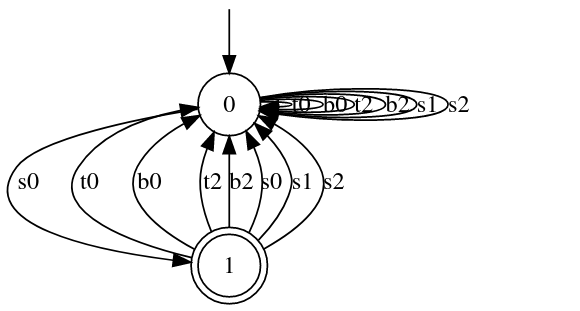
\includegraphics[width=0.4\linewidth]{res/minimalist_0}
  \caption{Automate $A_1$ lors du premier appel à l'oracle d'équivalence}\label{fig:fina1}
\end{figure}

\item L'automate $A_2$ de la figure \ref{fig:fina2} est proposé. Il est refusé et le contre-exemple $\gamma=\theta_1 t_{q_1}$ est retourné. En effet, il est accepté par $A_2$ mais ne peut pas être exécuté par $F$.
\begin{figure}[H]
  \centering
  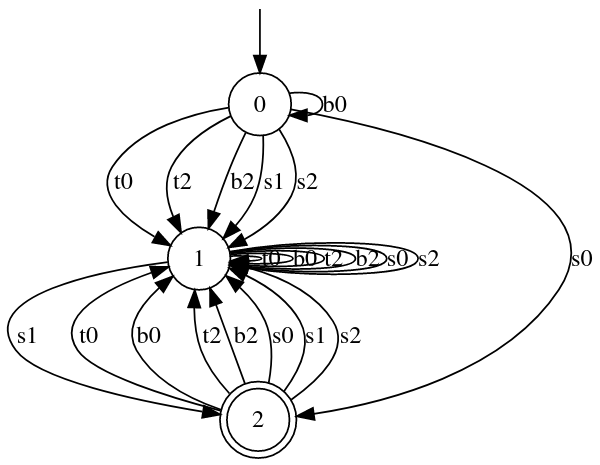
\includegraphics[width=0.4\linewidth]{res/minimalist_1}
  \caption{Automate $A_2$ lors du second appel à l'oracle d'équivalence}\label{fig:fina2}
\end{figure}

\item L'automate $A_3$ de la figure \ref{fig:fina3} est proposé. Aucun contre-exemple n'est trouvé contre $L(A)=AL(F)$. Alors, les ensembles $\mathcal{W}$ sont évalués.
\begin{figure}[H]
  \centering
  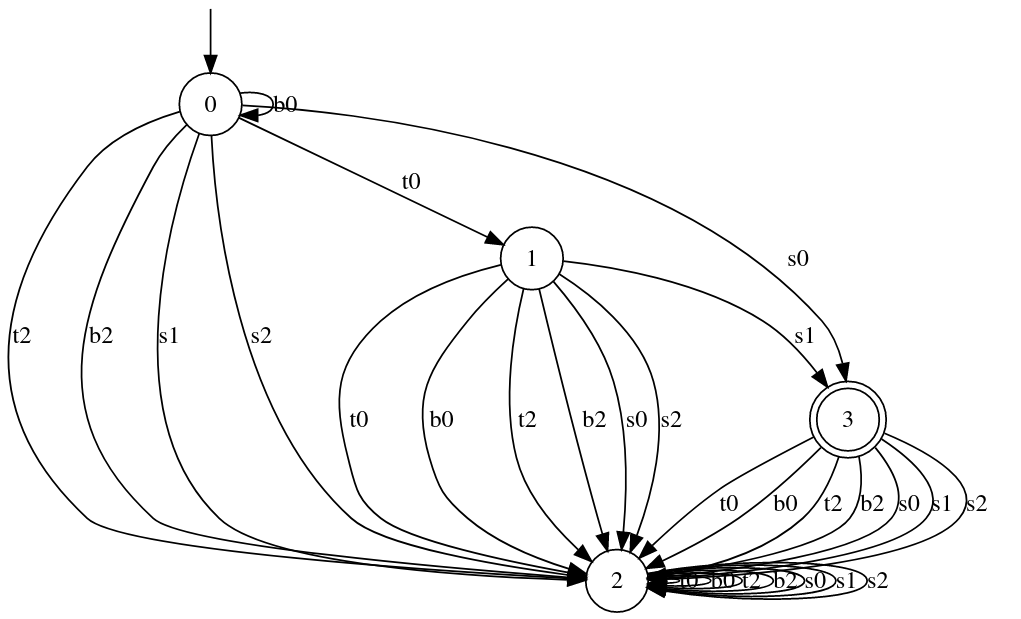
\includegraphics[width=0.6\linewidth]{res/minimalist_2}
  \caption{Automate $A_3$ lors du troisième appel à l'oracle d'équivalence}\label{fig:fina3}
\end{figure}

D'après $A_3$, il est possible de suivre le chemin $\gamma=\theta_1t_{q_1}$. Ce chemin passe par $q_1$. $F$ est alors déclaré comme à risque pour $\mathcal{W}_1$.

Par contre, aucun chemin valide ne passe par $q_2$. $F$ est alors déclaré comme sûr pour $\mathcal{W}_2$.
\end{enumerate}



\subsection{Exécution sans arrêt}

Pour cette troisième possibilité, l'algorithme qui ne s'arrête pas, l'automate à files $F$ utilisé est donné à la figure \ref{fig:fifo2}. Au nom des transitions près, indexées à partir de zéro, il s'agit du même automate à file que celui de la figure \ref{fig:fifo1}.

\begin{figure}[H]
  \centering
  \begin{tikzpicture}[->,>=stealth',shorten >=1pt,auto,node distance=2.5cm, semithick, bend angle=10]

    \tikzstyle{every state}=[circle]

    \node[initial,state] (A)                    {$q_0$};
    \node[state]         (B) [above right= 1cm and 3 cm of A] {$q_1$};
    \node[state]         (C) [below right= 1cm and 3 cm of A] {$q_2$};
    \node[state]         (D) [above right= 1cm and 3 cm of C] {$q_3$};

    \path
    (A) edge node {$\theta_0(a!0)$} (B)
    (A) edge node[below left] {$\theta_1(a!1)$} (C)
    (B) edge node {$\theta_3(a?0)$} (D)
    (B) edge[loop above] node {$\theta_2(b!1)$} (B)
    (C) edge node[below right] {$\theta_5(a?1)$} (D)
    (C) edge [loop below] node{$\theta_4(b!0)$} (C)
    (D) edge node[above] {$\theta_6(b?0)$} (A)
    ;
  \end{tikzpicture}
  \caption{Automate à files $F$}\label{fig:fifo2}
\end{figure}

Voici le suivi de l'exécution du programme jusqu'à ce qu'un motif récurrent émerge, suggérant que l'exécution ne s'arrête pas.

\begin{enumerate}
  \item L'automate $A_1$ acceptant le langage $L=\{t_{q_0}\}$ est proposé (figure \ref{fig:fina1}). Celui-ci est refusé et un contre-exemple est fourni : $\gamma=\theta_0 t_{q_1}$. En effet, $A_1$ n'accepte pas $\gamma$ alors qu'il existe bien une exécution valide de $F$ pour ce mot. C'est la même situation que dans la sous-section précédente.
  \begin{figure}[H]
    \centering
    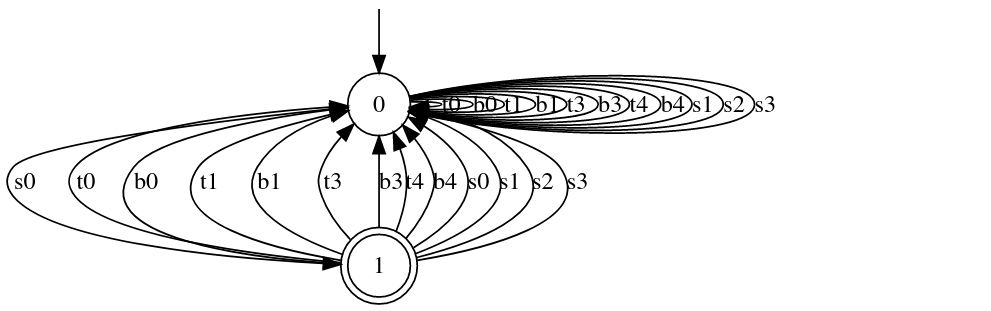
\includegraphics[width=0.6\linewidth]{res/andre_0}
    \caption{Automate $A_1$ lors du première appel à l'oracle d'équivalence}\label{fig:andre0}
  \end{figure}
  \item L'automate $A_2$ est proposé et refusé. Le contre-exemple $\gamma=\bt_0 t_{q_3}$ est retourné. En effet, le chemin $w=\theta_0.\theta_3$ est valide dans $F$, mène bien à $q_3$ et $\mathcal{A}(w)=\gamma$. $\gamma$ aurait dû être accepté par $A_2$.
  \item L'automate $A_3$ est proposé et refusé. Le contre-exemple $\gamma=\theta_3 t_{q_3}$ est retourné. $\gamma$ ne correspond à aucune exécution valide de $F$, ce mot ne devrait pas accepter par $A_3$.
  \item L'automate $A_4$ est proposé et refusé. Le contre-exemple $\gamma=\bt_1\theta_3 t_{q_3}$ est retourné, étant accepté par $A_4$ à tort.
  \item L'automate $A_5$ est proposé et refusé. Le contre-exemple $\gamma=\bt_1\bt_4\theta_4 t_{q_0}$ est retourné, le mot $\gamma$ n'étant pas accepté par $A_5$ alors qu'il devrait l'être.
  \item L'automate $A_6$ de la figure \ref{fig:andre6} est proposé. Il a été simplifié depuis l'automate original par souci de lisibilité.
  \begin{figure}[H]
    \centering
    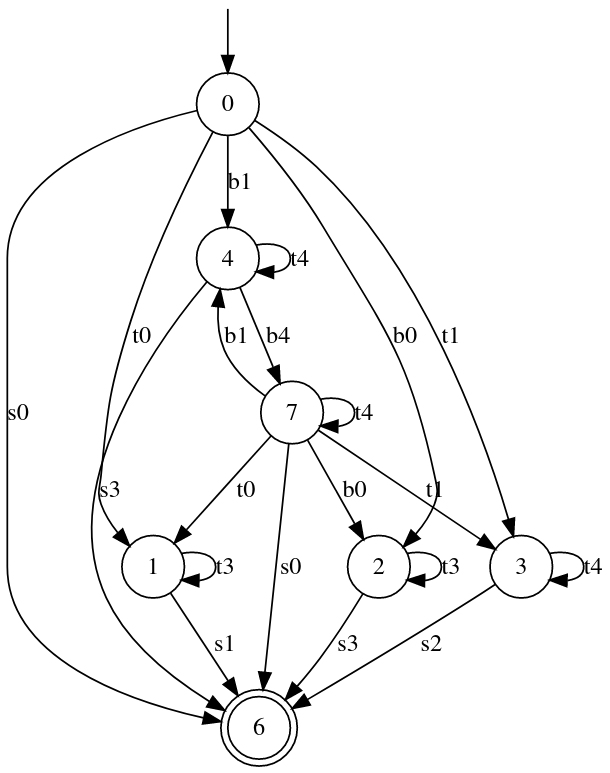
\includegraphics[width=0.4\linewidth]{res/andre_6}
    \caption{Automate $A_6$ lors du sixième appel à l'oracle d'équivalence}\label{fig:andre6}
  \end{figure}
  On peut déjà y remarquer une transition sur $\bt_4$ entre les états 4 et 7. Cependant, ce n'est pas suffisant. Un contre-exemple $\gamma=\bt_1\bt_4\bt_4\bt_0t_{q_0}$ est fourni. Le mot $\gamma$ n'est pas accepté par $A_6$ alors qu'il devrait l'être. Auquel cas, une exécution valide dans $F$ est : $w=\theta_1\theta_4\theta_4\theta_5\theta_6\theta_0\theta_3\theta_6$. $w$ est bien une exécution valide dans $F$ menant à $q_0$. De plus, $\mathcal{A}(w)=\gamma$.
  \item L'automate $A_7$ de la figure \ref{fig:andre7} est proposé. Il est également simplifié pour plus de lisibilité.
  Néanmoins, il reste plus complexe que $A_6$. En particulier, on peut noter l'apparition des états $8$ et $9$, servant à compter une utilisation de $\theta_4$ supplémentaire.
  Un contre-exemple $\gamma=\bt_1\bt_4\bt_4\bt_4\bt_0\bt_0t_{q_0}$ est fourni. Il est semblable au contre-exemple précédent. En réalité, il contient une utilisation de $\theta_4$ en plus.

  \begin{figure}[H]
    \centering
    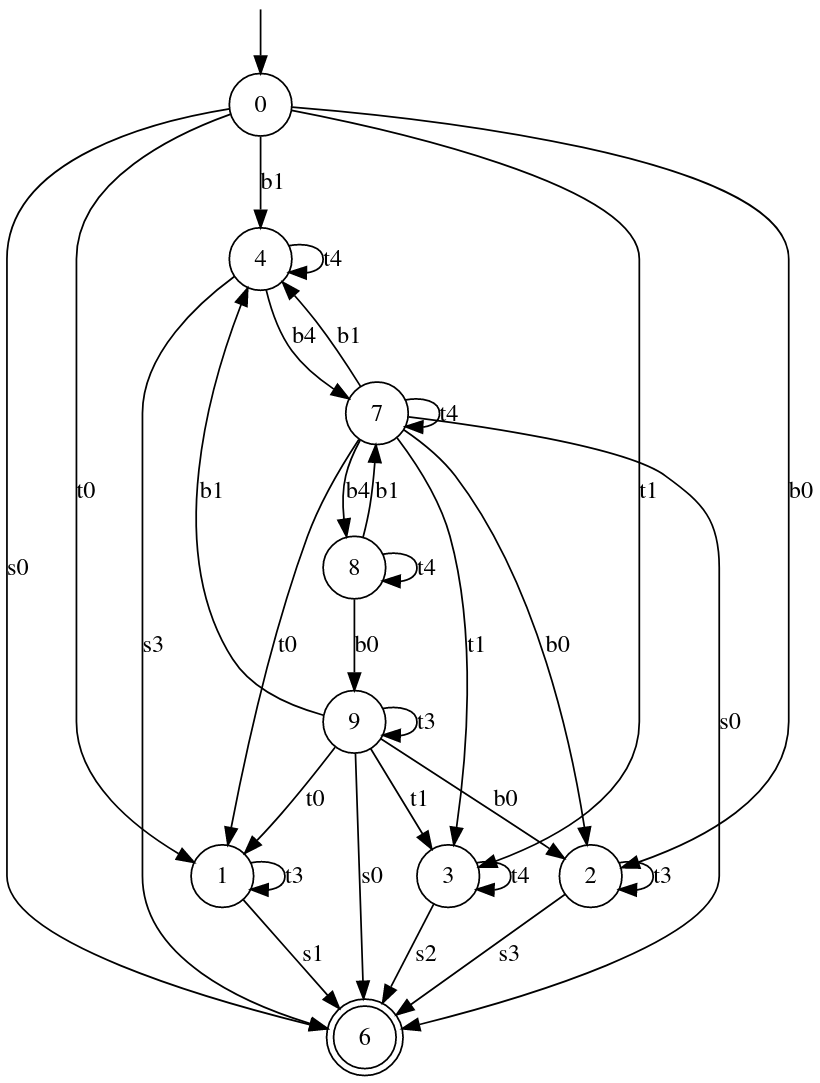
\includegraphics[width=0.6\linewidth]{res/andre_7}
    \caption{Automate $A_7$ lors du septième appel à l'oracle d'équivalence}\label{fig:andre7}
  \end{figure}

\end{enumerate}

À partir de là, l'automate se complexifie d'itération en itération, cherchant en vain à trouver un langage régulier permettant de garder le compte du nombre de transitions $\theta_4$ suivies. C'est un comportement cohérent au vu de l'automate $F$. Cet automate simple fait partie de la classe des automates à files pour lesquels la méthode LeVer est insuffisante.

